\input templates/header
\title[DS - Distributed Transactions]{\textbf{Distributed Algorithms}\\Distributed Transactions}

\graphicspath{{figs/13/}}

\setbeamercolor*{itemize item}{fg=darkred}


\newcommand{\TStart}{\textsc{tstart}}
\newcommand{\CKnow}{C_{\mathit{know}}}
\newcommand{\Transaction}{\mathit{transaction}}
\newcommand{\Decision}{\mathit{decision}}
\newcommand{\Participants}{\mathit{participants}}
\newcommand{\Vote}{\mathit{vote}}
\newcommand{\YES}{\textsc{yes}}
\newcommand{\NO}{\textsc{no}}
\newcommand{\VOTEREQUEST}{\textsc{voterequest}}
\newcommand{\VOTE}{\textsc{vote}}
\newcommand{\DECIDE}{\textsc{decide}}
\newcommand{\Now}{\textsf{now}}

\SetKw{TIMEOUT}{set timeout to}


\begin{document}

\FrameTitle{}
\FrameContent



%%%%%%%%%%%%%%%%%%%%%%%%%%%%%%%%%%%%%%%%%%%%%%%%%%%%%%%%%%%%%%%%%%%%%%%%%%

\section{Introduction and motivation}

%-------------------------------------------------------------------------
\begin{frame}{Introduction}
\begin{example}[Transfer money between two accounts]
\BI
\item Withdraw 200\euro\ from account 1
\item Deposit 200\euro\ to account 2
\EI
What happens if one of the operations is not performed?
\end{example}

\begin{definition}[Transaction]
The execution of a sequence of actions on a server that must be either
entirely completed or aborted, independently of other transactions
\end{definition}

Our goals:
\BI
\item We want to allow the execution of concurrent transactions, yet to
maintain consistency
\item We want to deal with the failure of either the server or the client
\EI

\end{frame}

%%%%%%%%%%%%%%%%%%%%%%%%%%%%%%%%%%%%%%%%%%%%%%%%%%%%%%%%%%%%%%%%%%%%%%%%%%

\section{Transactional models}
\subsection{ACID Properties}

%-------------------------------------------------------------------------
\begin{frame}{ACID Properties}
	
\BI
\item \alert{Atomicity}
	\BI
	\item Either all operations are completed or none of them is executed
	\EI
\item \alert{Consistency}
	\BI
	\item Application invariants must hold before and after a transaction; 
	\item during the transaction, invariants may be violated but this is not visible outside
	\EI
\item \alert{Isolation} (Serializability)
	  \BI
	  \item Execution of concurrent transactions should be equivalent (in effect) to a serialized execution
	  \EI
\item \alert{Durability}
	\BI
	\item Once a transaction commits, its effect are permanent
	\EI	
\EI
\end{frame}

%-------------------------------------------------------------------------
\begin{frame}{Transactional syntax}
	
\BI
\item Applications are coded in a stylized way:
	\BI
	\item begin transaction
	\item perform a series of read, write operations
	\item terminate by commit or abort
	\EI
\EI

\begin{Procedure}
\caption{Example of transaction (sketch)}
\TRANSACTION{$T$}{
$v_x \gets \Read("x")$\;
$v_y \gets \Read("y")$\;
$v_z \gets v_x + v_y$\;
$\Write("z", z)$\;
\COMMIT\;
}
\end{Procedure}

\end{frame}

%%%%%%%%%%%%%%%%%%%%%%%%%%%%%%%%%%%%%%%%%%%%%%%%%%%%%%%%%%%%%%%%%%%%%%%%%%
\subsection{Types of transactions}

%-------------------------------------------------------------------------
\begin{frame}{Flat transactions}
	
\BI
  \item Simplest, relatively easy to implement
  \item Their greatest strength (\alert{atomicity}) is also their weakness\\ (\emph{lack of flexibility})
\item Technical issues:
  \BI
  \item How to maintain isolation
  \item How to maintain atomicity + consistency
  \EI
\EI
\end{frame}

%-------------------------------------------------------------------------
\begin{frame}{Nested transactions}
	
  \BI
  \item Constructed from a number of sub-transactions
  \item Sub-transactions may run in parallel or in sequence
  \item The subdivision is \alert{logical}
  \item Flexibility
  \BI
  \item When a transaction fails, all its sub-transactions must fail too
  \item When a sub-transaction fails:
	\BI
	\item The parent transaction could fail
	\item Or, alternative actions could be taken
	\EI
  \EI
\item Example next slide
\EI
\end{frame}

%-------------------------------------------------------------------------
\begin{frame}{Nested transactions}

\begin{Procedure}
\caption{Example of nested transaction (sketch)}
\TRANSACTION{"book travel"}{
  \STARTTRANS "book flight"\; 
  \STARTTRANS "book hotel"\;
  \STARTTRANS "book car"\;
  \If{"book car" aborted}{
	\STARTTRANS "book bus"\;
  }
  \eIf{"book flight" \AND\ "book hotel" \AND\ ("book car" \OR\ "book bus") committed}{
    \COMMIT \;
  }{
      \ABORT \;
  }
} 

\end{Procedure}
\end{frame}

%-------------------------------------------------------------------------
\begin{frame}{Distributed transactions}

\BI
  \item Can be either flat or nested
  \item Operates on distributed data (multiple servers)
  \item Technical issues
  \BI
    \item Separate distributed algorithms are needed to handle
	\BI
	  \item locking of data in multiple distributed systems
	  \item committing data in an atomic way
	\EI
  \EI
\EI
\end{frame}

%-------------------------------------------------------------------------
\begin{frame}{Distributed transactions}
	
Example of distributed transaction (sketch)
\bigskip
\begin{columns}
\begin{column}{0.5\textwidth}
\begin{Procedure}
\caption{Site $A$, account $x$}
\TRANSACTION{$T$}{
  $v_x \gets \Read("x")$\; 
  $\Write("x", v_x + C)$\;
  \COMMIT\;
}
\vspace{1.10cm}
\end{Procedure}
\end{column}
\begin{column}{0.5\textwidth}
\begin{Procedure}
\caption{Site $B$, account $y$}
\TRANSACTION{$T$}{
  $v_y \gets read("y")$\;
  \If{$v_y \geq C$}{
	$\Write("y", v_y - C)$\;
	\COMMIT\;
  }{
	\ABORT\;
  }
}
\end{Procedure}
\end{column}
\end{columns}

\end{frame}

%-------------------------------------------------------------------------
\begin{frame}{Types of transactions}
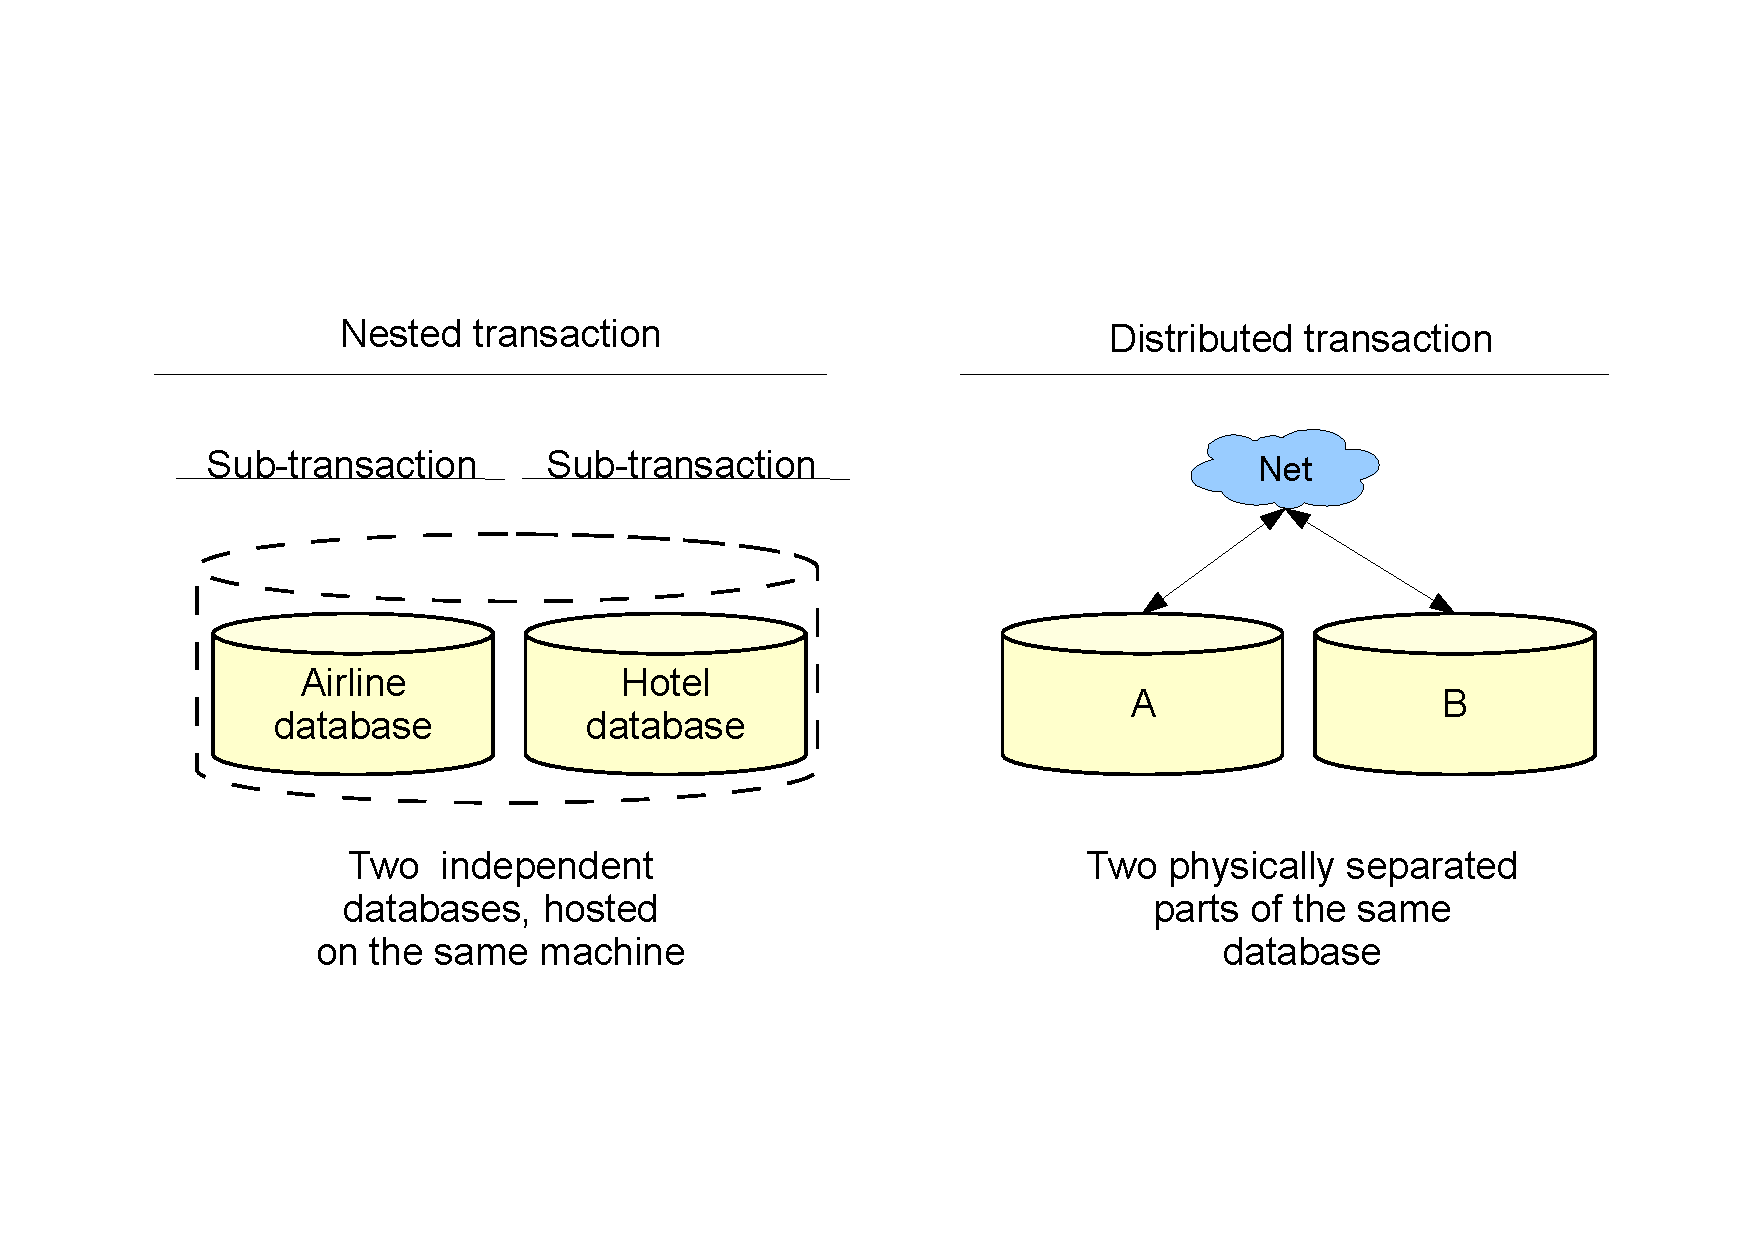
\includegraphics[width=\textwidth]{fig1-nested-distributed.pdf}
\end{frame}

%%%%%%%%%%%%%%%%%%%%%%%%%%%%%%%%%%%%%%%%%%%%%%%%%%%%%%%%%%%%%%%%%%%%%%%%%%
\section{Implementing transactions}

%-------------------------------------------------------------------------
\begin{frame}{Transactional system}
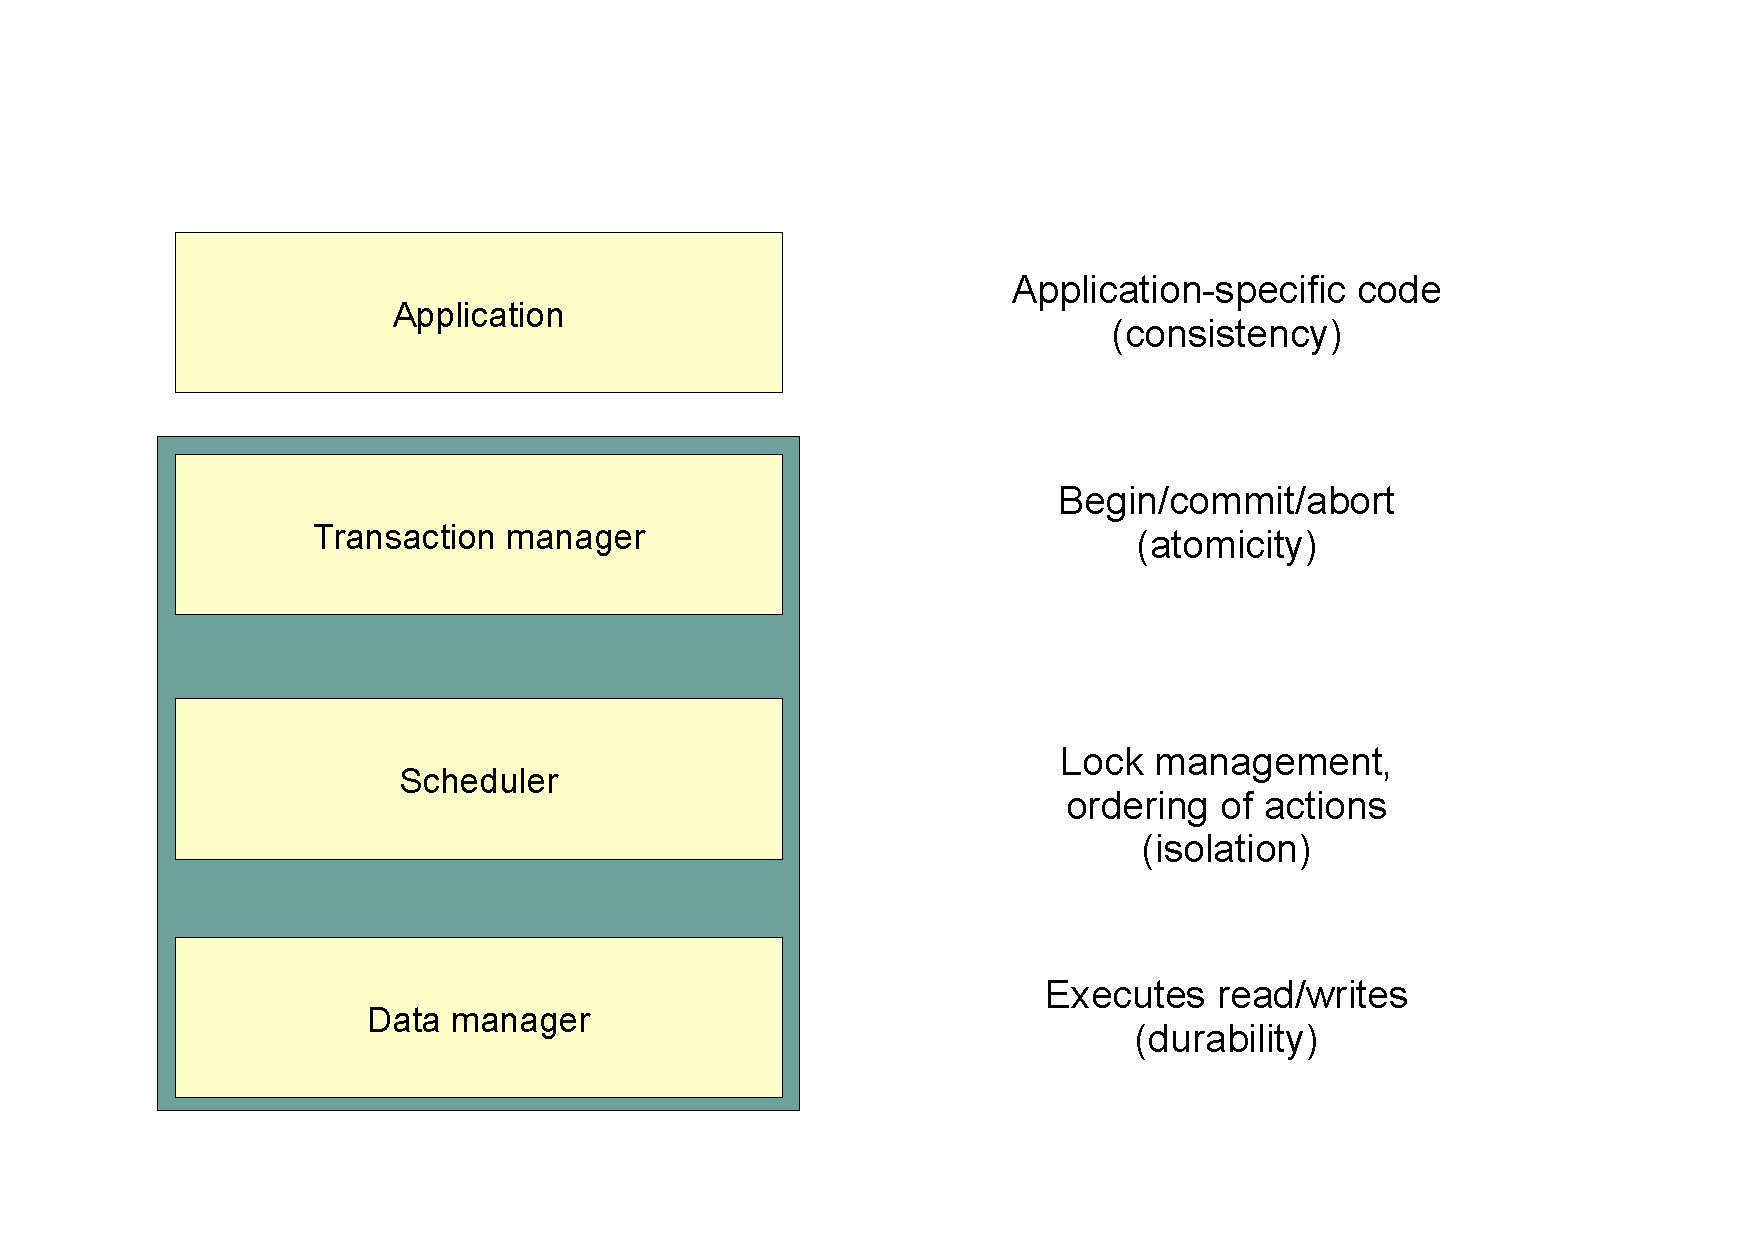
\includegraphics[width=\textwidth]{fig2-transactional.pdf}
\end{frame}

%-------------------------------------------------------------------------
\begin{frame}{Atomicity}
	
\BI
\item \alert{Private workspaces}
  \BI
  \item At the beginning, give the transaction a private workspace and copy all required objects
  \item Read/write/perform operations on the private workspace
  \item If all operations are successful, commit by writing the updates in the permanent record; otherwise abort
  \EI
\item How to extend this to a distributed system?
  \BI
  \item Each copy of the transaction on different server is given a private workspace
  \item Perform a distributed \alert{atomic commitment protocol}
  \EI
\EI

\end{frame}

%%%%%%%%%%%%%%%%%%%%%%%%%%%%%%%%%%%%%%%%%%%%%%%%%%%%%%%%%%%%%%%%%%%%%%%%%%
\subsection{Atomicity}


%-------------------------------------------------------------------------
\begin{frame}{Atomicity}
\BI
\item \alert{Write-ahead log}
  \BI
  \item Write operation / initial state / final state on a log
  \item Modify "real" data
  \EI
\item In case of commit
  \BI
  \item Mark operation as committed on the log
  \EI
\item In case of abort
  \BI
  \item Mark operation as aborted on the log
  \item Revert "real" data to the initial state
  \EI
\item How to extend this to a distributed system?
  \BI
  \item \alert{Distributed rollback recovery}
  \EI
\EI
\end{frame}

%-------------------------------------------------------------------------
\begin{frame}{Atomicity}
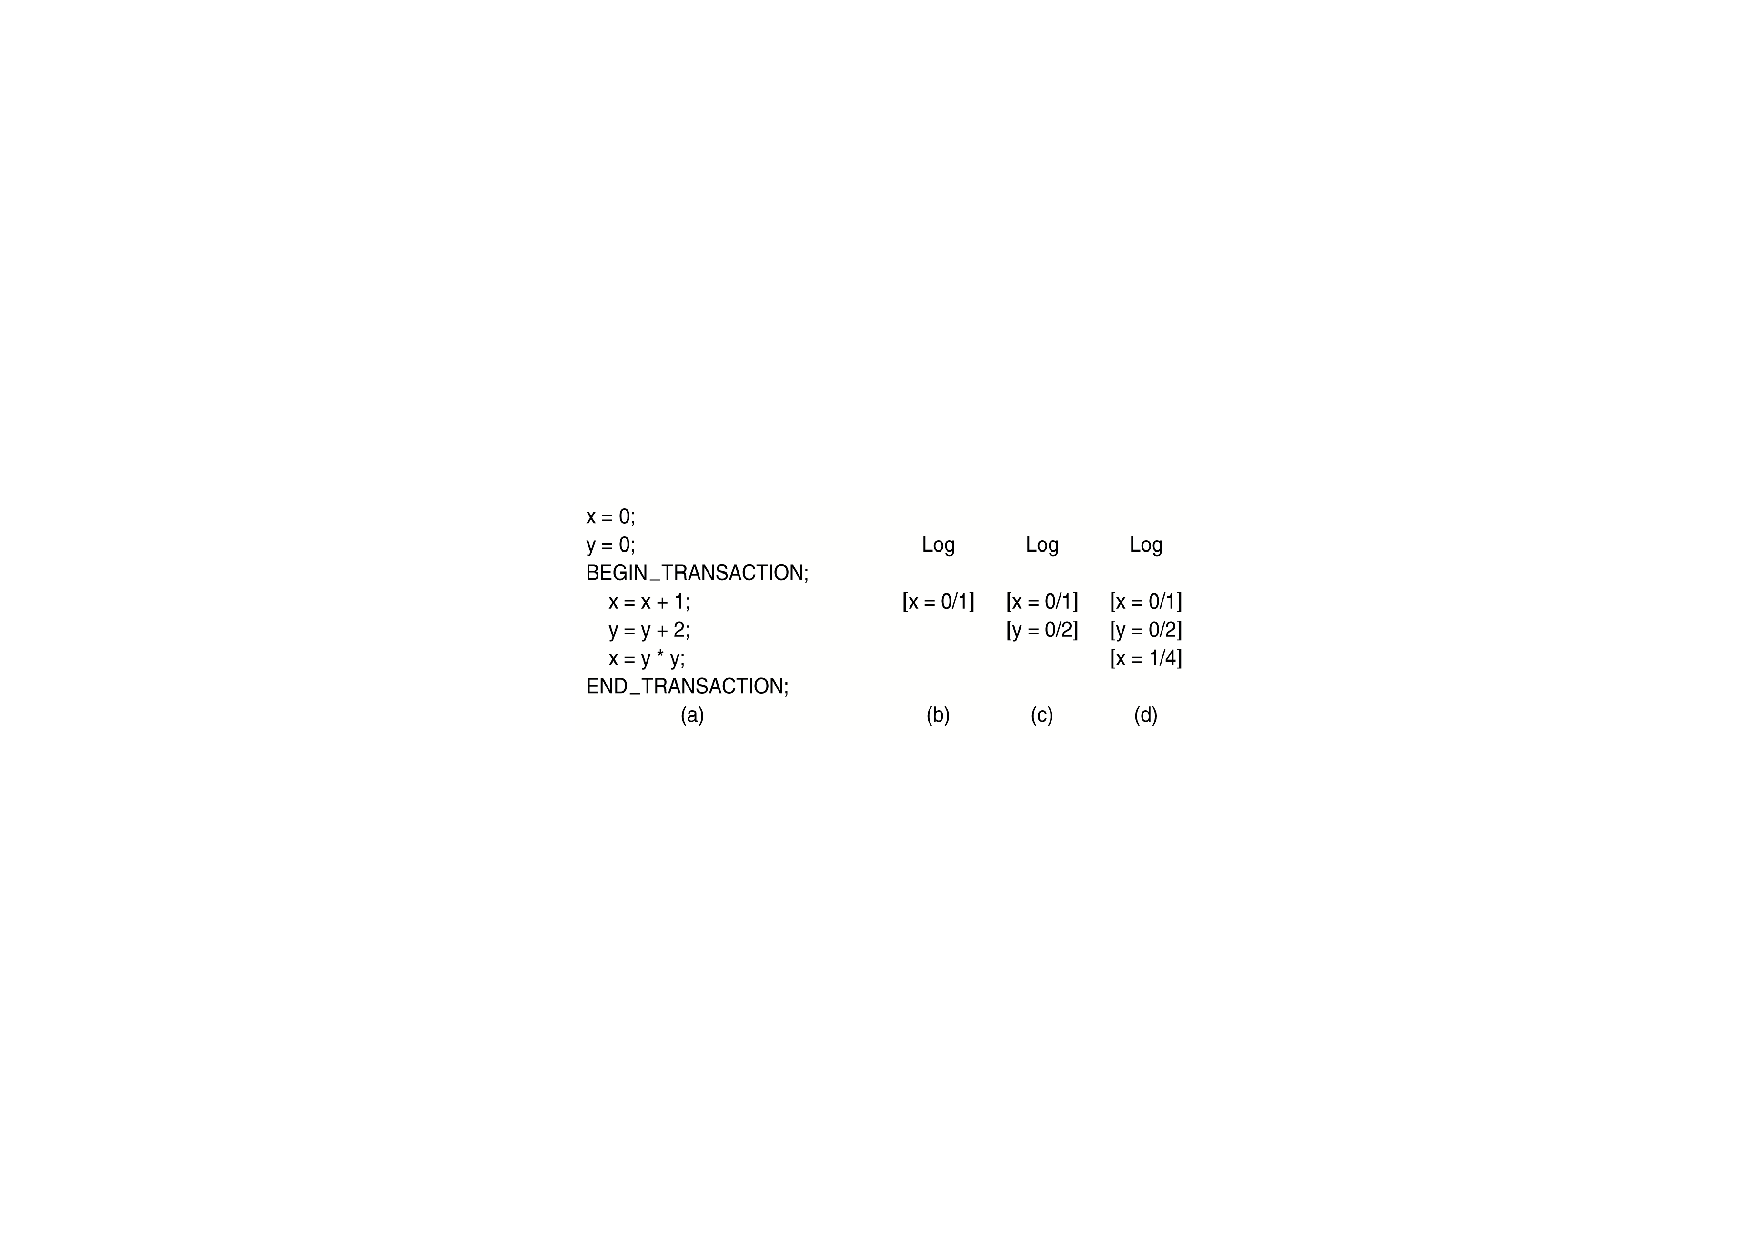
\includegraphics[width=0.8\textwidth]{fig3-log.pdf}
\end{frame}

%%%%%%%%%%%%%%%%%%%%%%%%%%%%%%%%%%%%%%%%%%%%%%%%%%%%%%%%%%%%%%%%%%%%%%%%%%
\subsection{Isolation}

%-------------------------------------------------------------------------
\begin{frame}{Isolation}

\BI
\item Isolation
  \BI
  \item Means that effect of the interleaved execution is indistinguishable from some possible serial execution of the committed transactions 
  \EI
\item Example:
  \BI
  \item $T_1$ and $T_2$ are interleaved but it "looks like" $T_2$ ran before $T_1$
  \EI
\item The idea:
  \BI
  \item Transactions can be coded to be correct if run in isolation, and yet will run correctly when executed concurrently (hence gain a speedup)
  \EI
\EI

\end{frame}

%-------------------------------------------------------------------------
\begin{frame}{Isolation}
	
\begin{columns}[T]
\begin{column}{0.5\textwidth}
\BI
\item Alice withdraws 250\euro\ from $X$ 
  \BI
  \item[1)] $\mathit{local} \gets \Read("x")$
  \item[2)] $\mathit{local} \gets \mathit{local} - 250$
  \item[3)] $\Write("x",\mathit{local})$
  \EI
\EI
\end{column}
\begin{column}{0.5\textwidth}
\BI
\item Bob withdraws 250\euro\ from $X$
  \BI
  \item[4)] $\mathit{local} \gets \Read("x")$
  \item[5)] $\mathit{local} \gets \mathit{local} - 250$
  \item[6)] $\Write("x",\mathit{local})$
  \EI
\EI

\end{column}
\end{columns}

\bigskip
\alert{What happens with the following sequences?}
\begin{overprint}
\onslide<1|handout:0>
\BI
\item 1-2-3-4-5-6
\item 4-5-6-1-2-3
\item 1-4-2-5-3-6
\item 1-2-4-5-6-3
\EI
\onslide<2|handout:1>
\BI
\item 1-2-3-4-5-6 \qquad Correct
\item 4-5-6-1-2-3 \qquad Correct
\item 1-4-2-5-3-6 \qquad Lost update
\item 1-2-4-5-6-3 \qquad Lost update
\EI
\end{overprint}
\end{frame}


   

%-------------------------------------------------------------------------
\begin{frame}{Isolation}
\begin{overprint}
\onslide<1|handout:1>
\begin{figure}	
	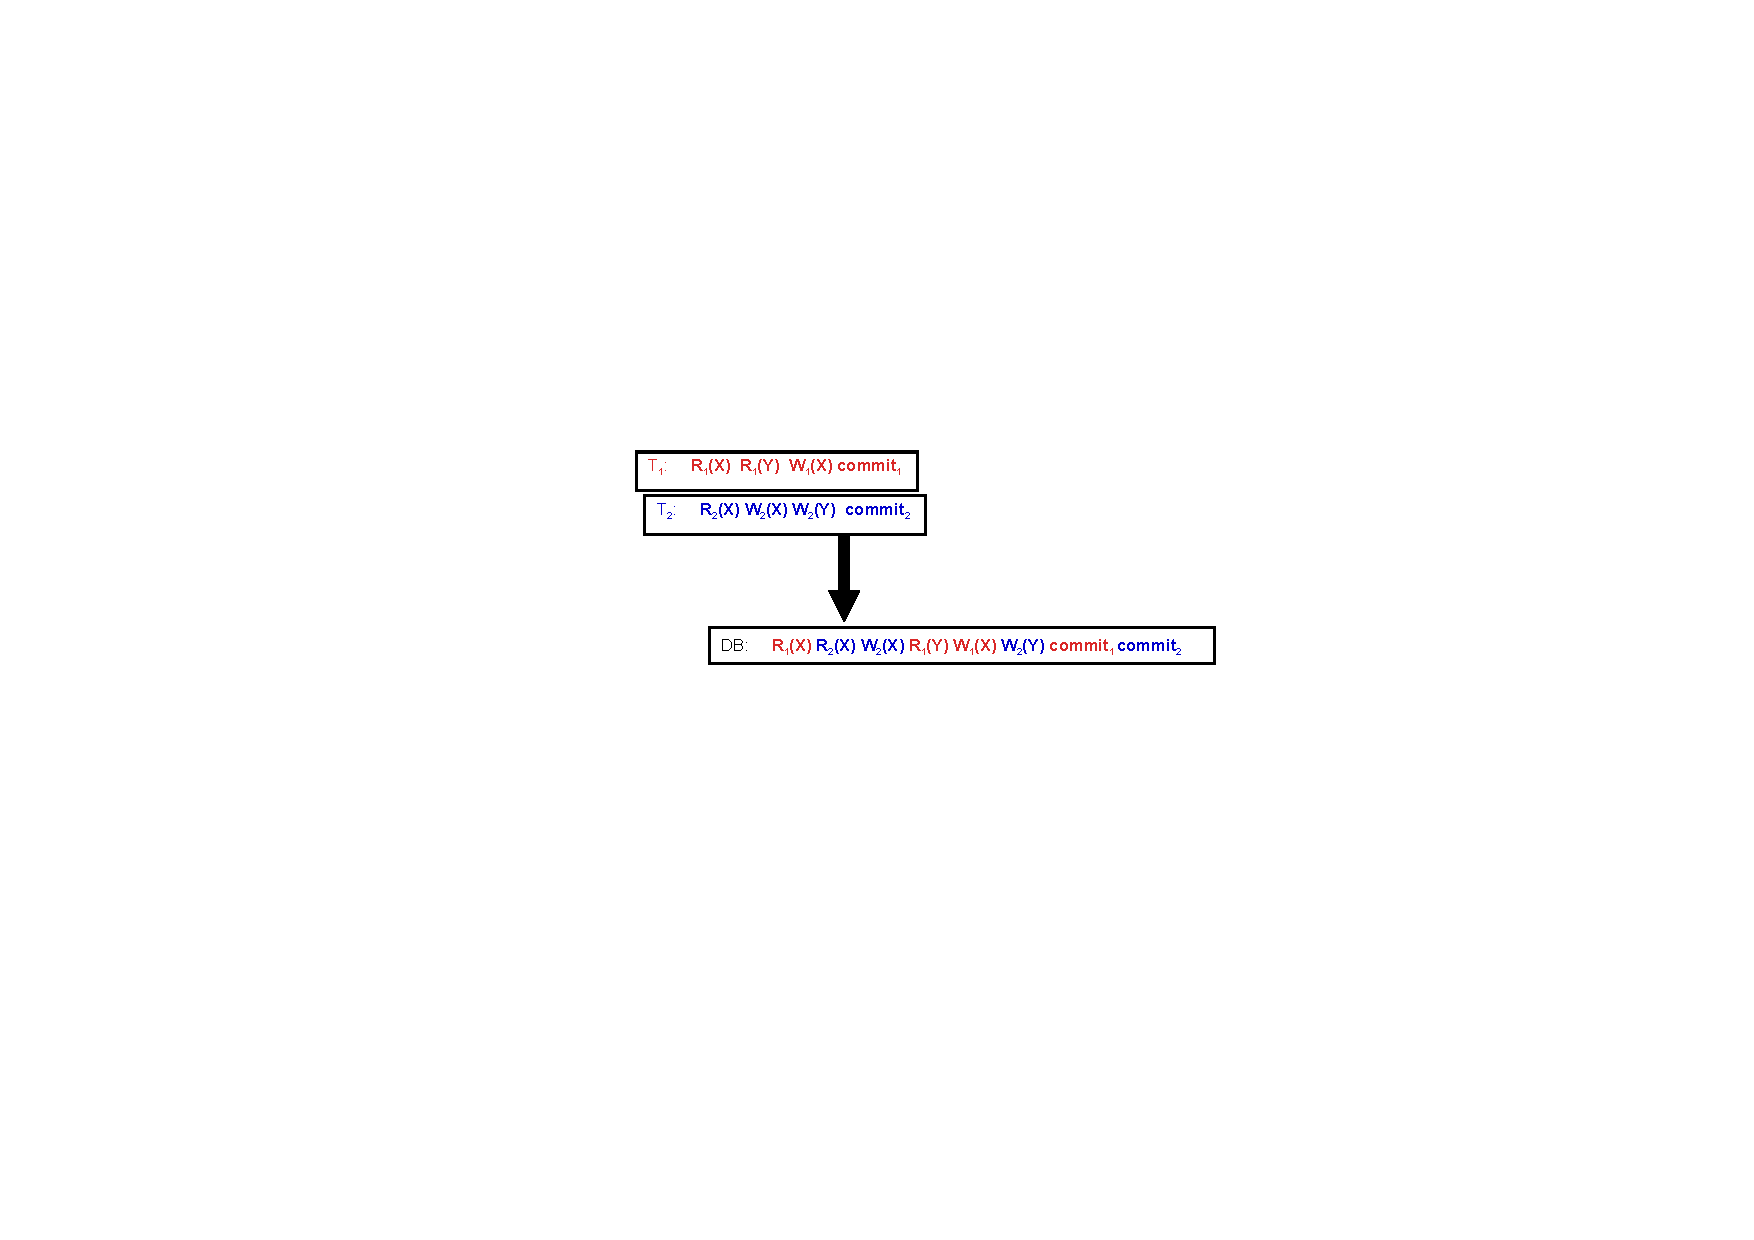
\includegraphics[width=\textwidth,page=1]{fig4-isolation.pdf}
\end{figure}
\onslide<2|handout:2>
\begin{figure}	
	\includegraphics[width=\textwidth,page=2]{fig4-isolation.pdf}
\end{figure}
\onslide<3|handout:3>
\begin{figure}	
	\includegraphics[width=\textwidth,page=3]{fig4-isolation.pdf}
\end{figure}
\end{overprint}

\end{frame}

%-------------------------------------------------------------------------
\begin{frame}{Locking}
	
Unlike other kinds of distributed systems, transactional systems typically lock the data they access

\bigskip
\begin{columns}[T]
\begin{column}{0.5\textwidth}
\BI
\item \alert{Lock coverage}
  \BI 
  \item suppose that transaction $T$ will access object $x$
  \item $T$ must gets a lock that "covers" $x$
  \EI
\EI
\end{column}
\begin{column}{0.5\textwidth}
\BI
\item We could have one lock   
  \BI
  \item \ldots per object
  \item \ldots for the whole database   
  \item \ldots for a category of objects   
  \item \ldots per table
  \item \ldots per row
  \EI
\item All transactions must obey the same rules!
\EI
\end{column}
\end{columns}

\end{frame}

%-------------------------------------------------------------------------
\begin{frame}{Strict 2-Phase locking (2-PL)}
\BI
\item $1^{\textrm{st}}$ phase ("growing")
  \BI
  \item Whenever the scheduler receives an operation $\mathit{operation}(T,x)$
  \item If $x$ is already owned by a conflicting lock:
    \BI
    \item the operation (and the transaction) is delayed   Otherwise:
    \item the lock is granted
	\EI
  \item Obtain all the locks it needs while it runs and hold onto them even if no longer needed!
  \EI
\item $2^{\textrm{nd}}$ phase ("shrinking")
  \BI
  \item release locks only after making commit/abort decision and only after updates are persistent
  \EI
\EI
\end{frame}

%-------------------------------------------------------------------------
\begin{frame}{2-PL implies Serializability}
\BI
\item Suppose that $T'$ performs an operation that conflicts with an operation that $T$ has done
  \BI
  \item e.g., $T'$ will update data item $x$ that $T$ read or updated
  \item e.g., $T$ updated item $y$ and $T'$ will read it
  \EI
\item $T$ must have had a lock on $x/y$ that conflicts with the lock that $T'$ wants
  \BI
  \item $T$ won't release it until it commits or aborts
  \item So $T'$ will wait until $T$ commits or aborts
  \EI
\item Note: 2-PL may cause deadlocks; usual techniques apply
\EI
\end{frame}


%%%%%%%%%%%%%%%%%%%%%%%%%%%%%%%%%%%%%%%%%%%%%%%%%%%%%%%%%%%%%%%%%%%%%%%%%%
\subsection{Durability}

%-------------------------------------------------------------------------
\begin{frame}{Durability: Lampson's stable storage}

\BI
\item Maintain two copies of object $A$ ($A_0$ and $A_1$) plus two timestamps and checksums (different disks)
\item Failure may happen at anytime between the six operations
\EI

{\footnotesize

\begin{columns}[T]
\begin{column}{0.32\textwidth}
\begin{center}
\alert{Writing}
\end{center}
\vspace{-12pt}
\begin{Procedure}
\caption{$\textsc{update}(A, x)$}
$A_0 \gets x$\;
$T_0 \gets \textsf{now}()$\;
$S_0 \gets \textsf{checksum}(x, t_0)$\;
$A_1 \gets x$\;
$T_1 \gets \textsf{now}()$\;
$S_1 \gets \textsf{checksum}(x, t_1)$\;
\end{Procedure}
\end{column}
\hfill
\begin{column}{0.67\textwidth}
\begin{center}
\alert{Recovery}
\end{center}
\vspace{-12pt}
\begin{Procedure}
\caption{$\textsc{read}(A)$}
\If{$S_0 = \textsf{checksum}(A_0, T_0) \wedge S_1 = \textsf{checksum}(A_1, T_1)$}{
  \lIf{$T_0>T_1$}{
  	\Return $A_0$
  }
  \hspace{1.7cm}\lElse{
  	\Return $A_1$
  }
}
\If{$S_0 = \textsf{checksum}(A_0, T_0) \wedge S_1 \neq \textsf{checksum}(A_1, T_1)$}{
  	\Return $A_0$\;
}
\If{$S_0 \neq \textsf{checksum}(A_0, T_0)  \wedge S_1 = \textsf{checksum}(A_1, T_1)$}{
  	\Return $A_1$\;
}
\end{Procedure}
\end{column}
\end{columns}
}
\end{frame}

%%%%%%%%%%%%%%%%%%%%%%%%%%%%%%%%%%%%%%%%%%%%%%%%%%%%%%%%%%%%%%%%%%%%%%%%%%
\section{From centralized to distributed}

\subsection{Isolation}

%-------------------------------------------------------------------------
\begin{frame}{Distributed locking}

\BI
\item \alert{Centralized 2-PL}
  \BI
  \item A single site is responsible for granting and releasing locks
  \item Each scheduler communicates with this centralized scheduler
  \item Issues: bottleneck, central point of failure
  \EI
\item  \alert{Primary 2-PL}
  \BI
  \item Each data item is assigned to a "primary" server
  \item Each scheduler communicates with the scheduler of the primary
  \item Issues: central points of failure
  \EI
\item \alert{Distributed 2-PL}
  \BI
  \item Locking is done in a decentralized way; messages are exchanged through reliable multicast
  \EI
\EI
\end{frame}

%-------------------------------------------------------------------------
\begin{frame}{Failures on centralized system}
\BI
\item If application crashes: 
 \BI 
  \item Treat as an abort 
  \EI
\item If transactional system crashes:
 \BI 
 \item Abort non-committed transactions, but committed state is durable
 \EI
\item Aborted transactions:
  \BI
  \item Leave no effect, either in database itself or in terms of indirect side-effects
  \item Only need to consider committed operations in determining serializability
  \EI
\EI
\end{frame}

\subsection{Distributed commitment}

%-------------------------------------------------------------------------
\begin{frame}{Distributed commit problem}
\BI
\item \alert{Atomic commitment}
  \item The distributed commit problem involves having an operation being performed by a distributed set of participants
\item Two protocols
  \BI
  \item \alert{Two-phase commit} (2PC)
    \BI
    \item blocking, efficient
    \item Jim Gray (1978)
    \EI
  \item \alert{Three-phase commit} (3PC)
    \BI
    \item non-blocking
    \item Dale Skeen (1981)
	\EI
  \EI
\item Implementations based on a coordinator
\EI
\end{frame}

%-------------------------------------------------------------------------
\begin{frame}{System model}
\BI
\item Fixed set of participants, known to all
\item No message losses
\item Synchronous communication: all messages arrive in $\delta$ time units
\item $\Delta_b$-timeliness: it is possible to build a broadcast primitive such that all messages arrive in $\Delta_b$ time units
\item Clocks exists
  \BI
  \item they are not required to be synchronized
  \item they may drift from real-time
  \EI
\bigskip
\item Which systems:
  \BI
  \item local area networks
  \EI
\EI
\end{frame}

%-------------------------------------------------------------------------
\begin{frame}{Generic Participant}	
\begin{Procedure}
\caption{Executed by the invoker}
\SEND $\langle \TStart, \Transaction, \Participants \rangle$ \TO\ $\Participants$\;
\end{Procedure}

\begin{Procedure}
\caption{Executed by all participants (including the invoker)}
\UPON{receipt of $\langle \TStart, \Transaction, \Participants \rangle$}{
  $\CKnow \gets \Now()$\;
  \{  Perform operations requested by $\Transaction$ \}\;
  \eIf{willing and able to make updates permanent}{
    $\Vote = \YES$\;
  }{
    $\Vote = \NO$\;
  }
  $\textsf{AtomicCommitment}(\Transaction, \Participants)$\;
}
\end{Procedure}
\end{frame}

%-------------------------------------------------------------------------
\begin{frame}{Coordinator selection}

\begin{block}{\alert{Coordinator axioms}}
\BI
\item[AX1] At most one participant will assume the role of coordinator 
\item[AX2] If no failures occur, one participant will assume the role of coordinator
\item[AX3] There exists a known constant $\Delta_c$ such that no participant assumes the role of coordinator more than $\Delta_c$ time units after the beginning of the transaction
\EI
\end{block}
\end{frame}

%-------------------------------------------------------------------------
\begin{frame}{Specification}
\begin{block}{\alert{Atomic commitment}}
\BI
\item[AC1] All participants that decide reach the same decision
\item[AC2] If any participant decides commit, then all participants must have voted yes
\item[AC3] If all participants vote yes and no failures occur, then all participants decide commit
\item[AC4] Each participant decides at most once
\EI
\end{block}
\end{frame}

%-------------------------------------------------------------------------
\begin{frame}{Atomic commitment}

A generic algorithm – \emph{Atomic Commitment Protocol} (ACP)
\BI
  \item Based on a generic broadcast primitive
  \item By "plugging in" different versions of broadcast we obtain different versions of ACP
\EI

\bigskip
Three phases:
\BI
\item \textbf{Phase 1}:
  The coordinator asks for votes yes/no from participants and take a commit/abort decision 
\item \textbf{Phase 2}:
  The coordinator disseminates the decision
\item \textbf{Phase 3}:
  Termination protocol; we'll see	
\EI
\end{frame}

%-------------------------------------------------------------------------
\begin{frame}{Atomic Commitment Protocol}

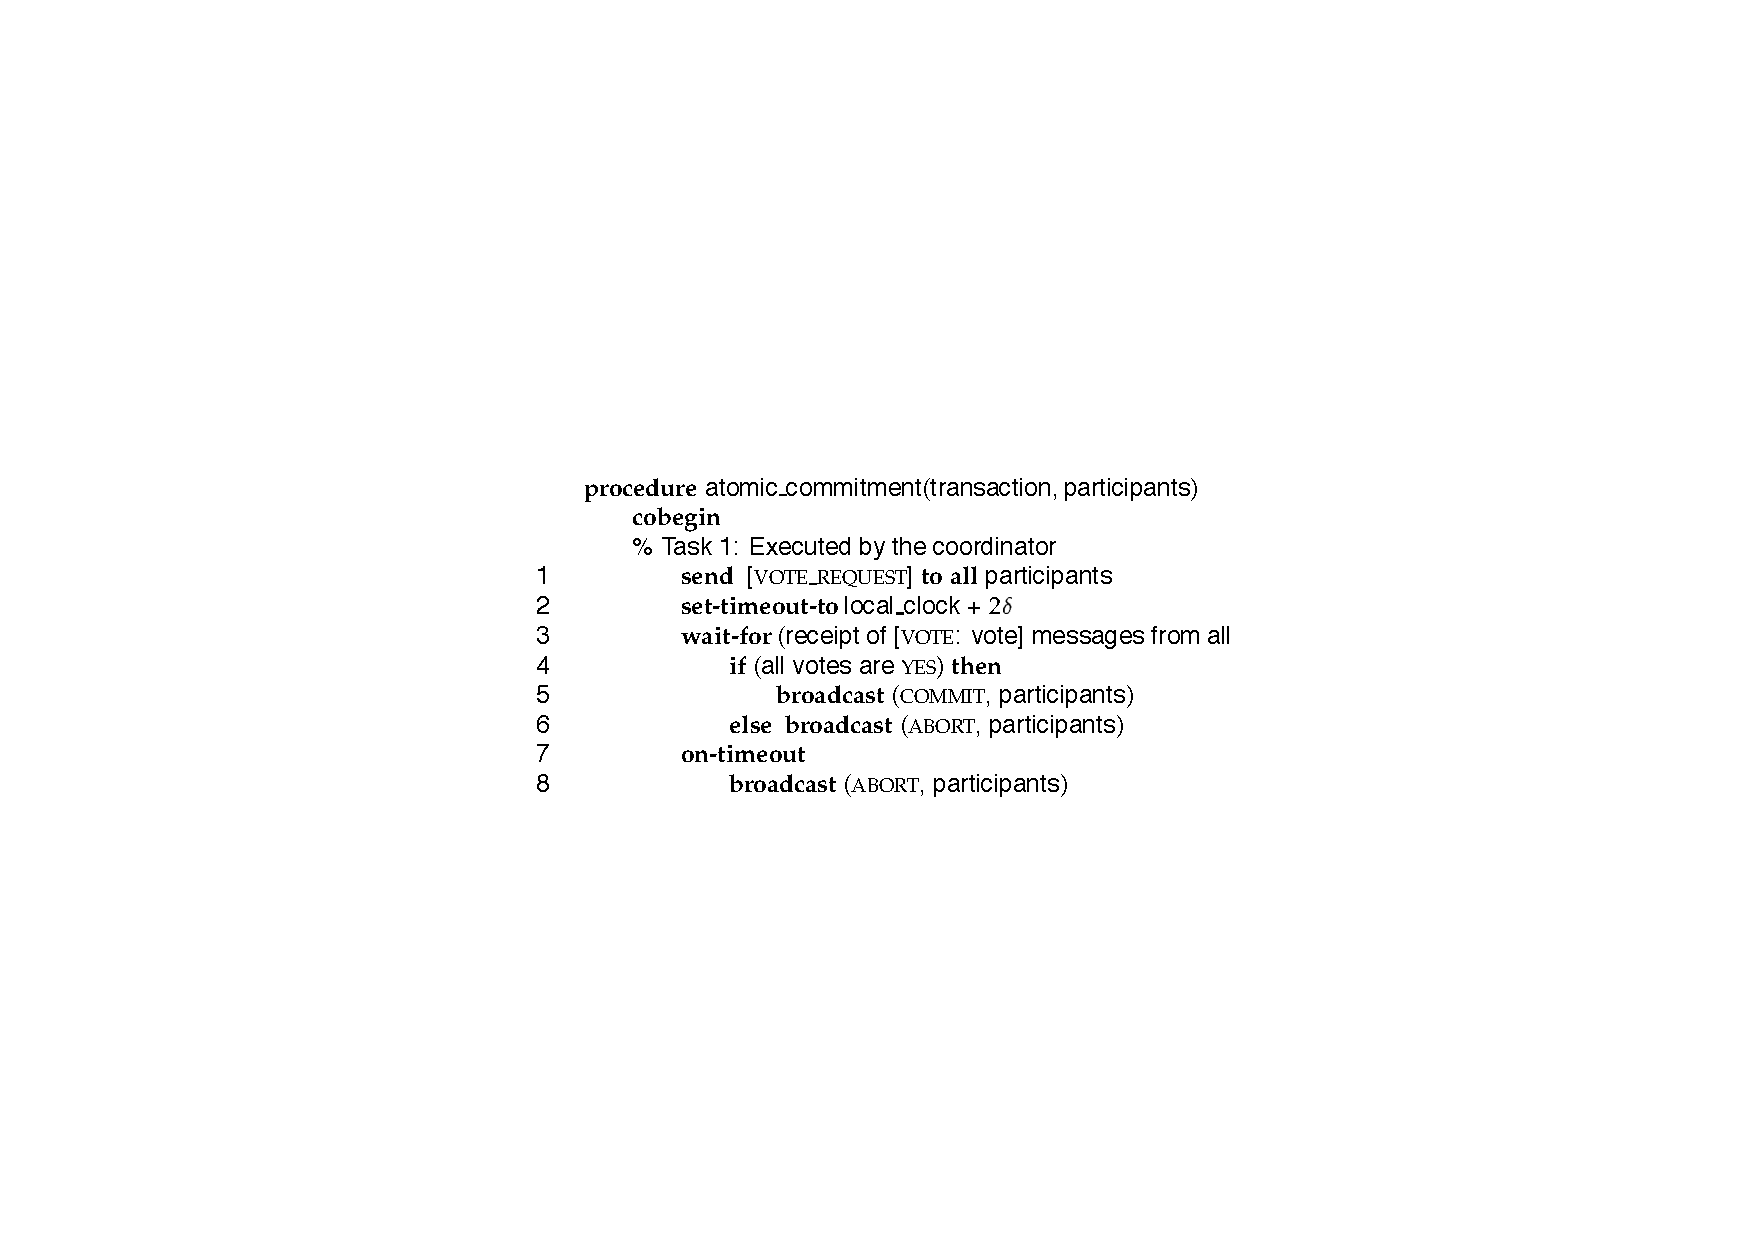
\includegraphics[width=\textwidth]{alg1.pdf}

\end{frame}



% \begin{frame}{Atomic Commitment Protocol}
%
%
% \begin{Procedure}
% \caption{Executed by the coordinator}
% \SEND $\langle \VOTEREQUEST \rangle$ \TO\ $\Participants$\;
% \TIMEOUT {$\Now()+ 2 \delta$}\;
% \eWAITFOR{receipt of $\langle \VOTE: \Vote \rangle$ from all $\Participants$}{
%   \eIf{all votes are \YES}{
%     \BROADCAST $\langle \DECIDE, \COMMIT \rangle$ \TO\ $\Participants$\;
%   }{
%     \BROADCAST $\langle \DECIDE, \ABORT \rangle$ \TO\ $\Participants$\;
%   }
% }{
%     \BROADCAST $\langle \DECIDE, \ABORT \rangle$ \TO\ $\Participants$\;
% }
% \end{Procedure}
%
%
% \end{frame}

%-------------------------------------------------------------------------
\begin{frame}{Atomic Commitment Protocol}

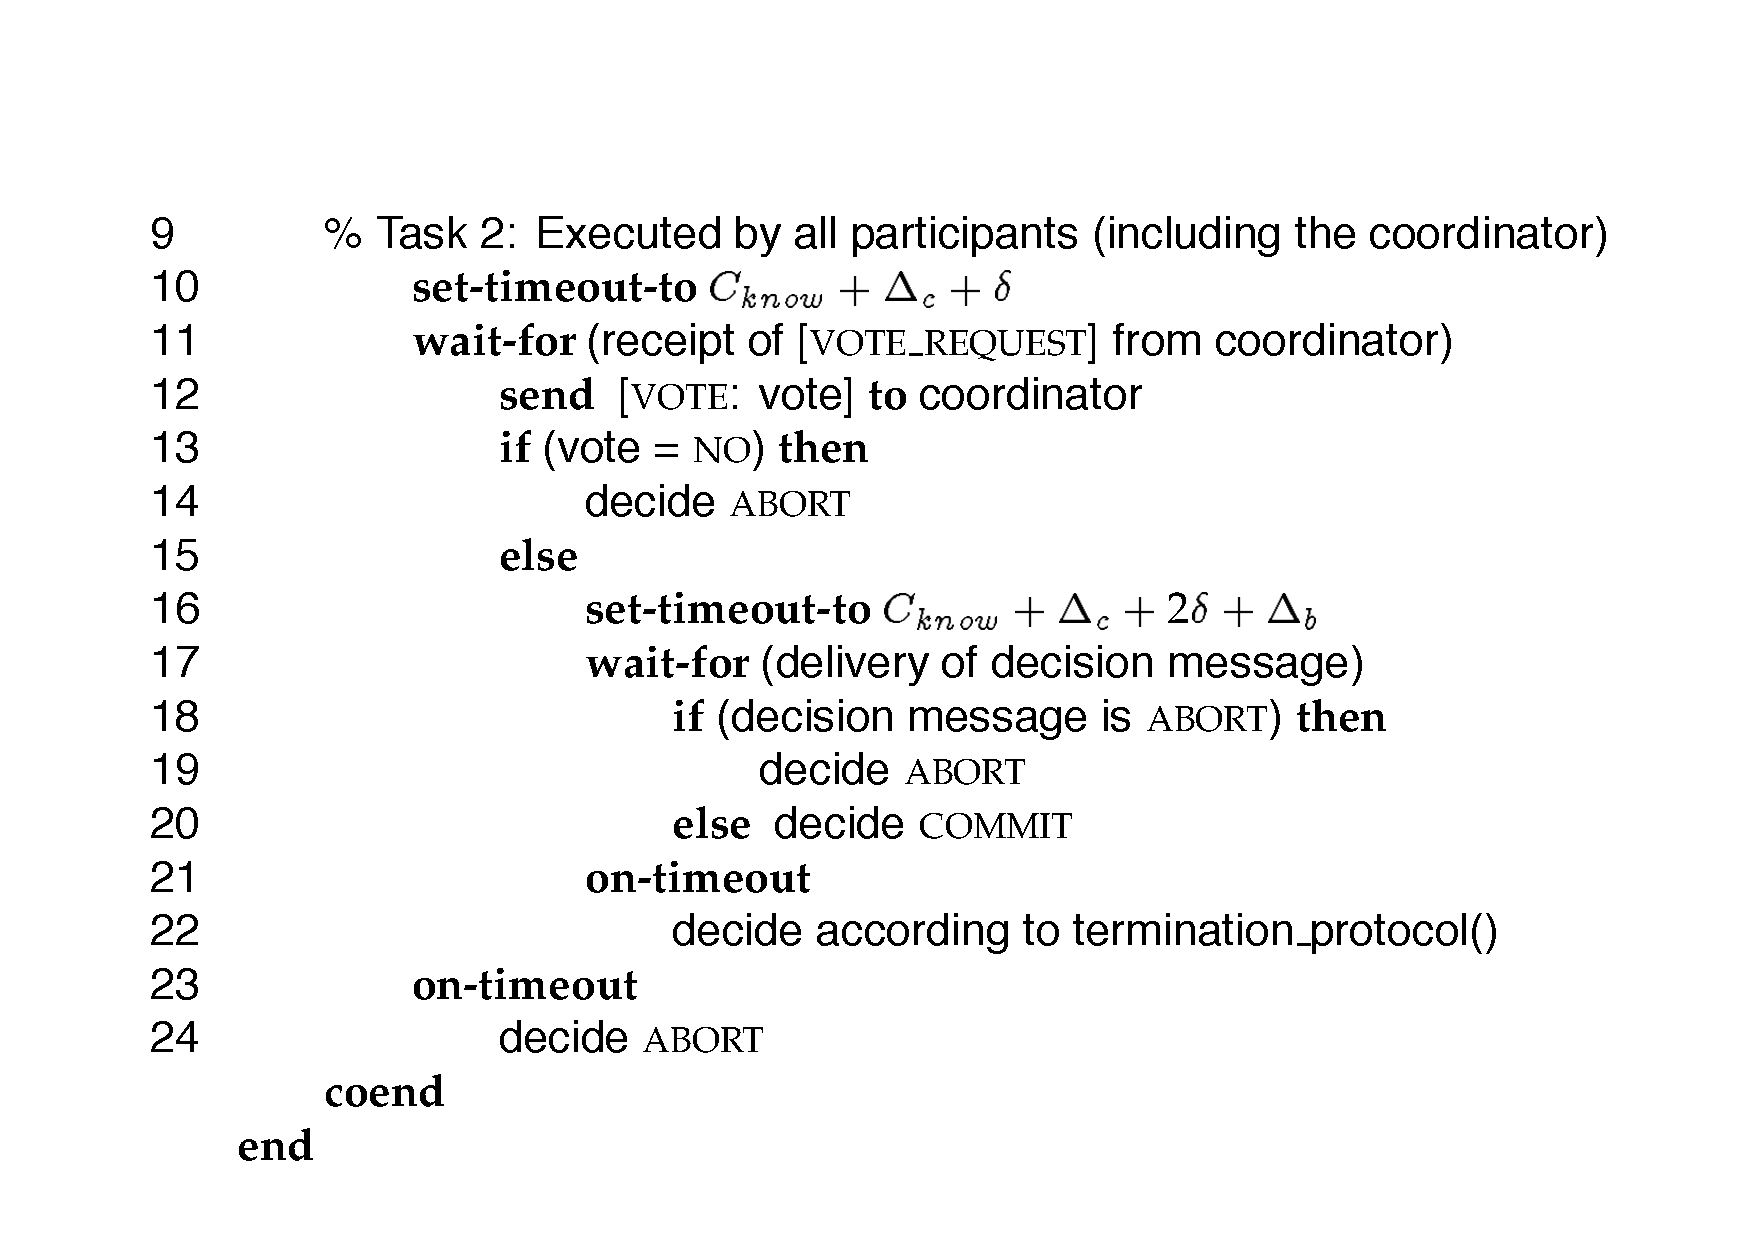
\includegraphics[width=\textwidth]{alg2.pdf}

% \begin{Procedure}
% \caption{Executed by all (including the coordinator)}
% \TIMEOUT $\CKnow + \Delta_c + \delta$\;
% \WAITFOR{receipt of $\langle \VOTEREQUEST \rangle$ from coordinator}{
%   \SEND $\langle \VOTE, \Vote \rangle$ \TO\ coordinator\;
%   \eIf{$\Vote=\NO$}{
%     $\Decide(\ABORT)$\;
%   }{
%     \TIMEOUT $\CKnow + \Delta_c + 2\delta + \Delta_b$\;
% 	\WAITFOR{delivery of $\langle \DECIDE, \Decision \rangle$}{
% 	  $\Decide(\Decision)$\;
% 	}{
% 	  \{ decide according to termination protocol \}
% 	}
%   }
% }{
%   $\Decide(\ABORT)$\;
% }
% \end{Procedure}
\end{frame}

%-------------------------------------------------------------------------
\begin{frame}{Terminating Best-Effort Broadcast}
 
\begin{definition}[TBEB1 - Validity]
If $p$ and $q$ are correct, then every message B-broadcast by $p$ is eventually delivered by $q$
\end{definition}

\smallskip
\begin{definition}[TBEB2 - Uniform Integrity]
$m$ is delivered by a process at most once, and only if it was previously broadcast
\end{definition}

\smallskip
\begin{definition}[TBEB3 - $\Delta_b$-Timeliness]
All messages arrive in $\Delta_b$ time units since the time they were sent
\end{definition}
\end{frame}

%-------------------------------------------------------------------------
\begin{frame}[shrink=5]{ACP - TBEB}
\BI
\item The ACP algorithm with a best-effort broadcast implementation
\item It happens to be equivalent to 2PC
\EI

\bigskip
{
\noindent
\def\arraystretch{1.5}
\begin{tabular}{|P{0.45\textwidth}|P{0.48\textwidth}|}
\hline
\textbf{AC1}: All participants that decide reach the same decision & See next page\newline (too complex to fit in this box!) \\\hline
\textbf{AC2}: If any participant decides \COMMIT, then all participants must have voted \YES & From the structure of the program (the coordinator must have received yes from all participants)  \\\hline
\textbf{AC3}: If all participants vote \YES\ and no failures occur, then all participants decide \COMMIT & Given reliable communication, no failure, synchrony, all messages arrives before deadlines \\\hline
\textbf{AC4}: Each participant decides at most once & From the algorithm structure (decide op. are mutually exclusive) \\\hline
\end{tabular}
}
\end{frame}
%-------------------------------------------------------------------------
\begin{frame}{Proof of AC1, by contradiction}
\BI
\item[1.] Let $p$ decide commit, let $q$ decide \ABORT. By AC4, $p \neq q$
\item[2.] $p$ must have received a broadcast from a coordinator $c$
	\BI
	\item[2.1] By AC2, $c$ must have received votes \YES\ from all, including $q$
	\EI
\item[3.] A process decide \ABORT\ in lines 14,19, 24 
	\BI
	\item[3.1] Line 14 is excluded by 2.1
	\item[3.2] Line 24 is excluded by 2.
	\EI
\item[4.] So $q$ must have delivered a message \ABORT\ in line 19
\item[5.] But this message must have been sent by a coordinator different from
$c$; but this is a contradiction with AX1 (unique coordinator)
\EI
\end{frame}

%-------------------------------------------------------------------------
\begin{frame}{Blocking vs non-blocking}
	
\BI
\item In some cases, a termination protocol is invoked
\item Informally, tries to contact other participants to learn a decision
	\BI 
	\item For example:
		\BI
		\item if a process has already decided, copy the decision
		\item if a process has not voted, decide \ABORT\
		\EI
	\EI
\item But consider this scenario:
	\BI
		\item the coordinator crashes during the broadcast of a decision
		\item all faulty participants decide and then crash
		\item all correct participants have previously voted \YES, and they do not deliver a decision
	\EI
\item ACP-TBEB is blocking in this scenario
\EI


\end{frame}

%-------------------------------------------------------------------------
\begin{frame}{Blocking vs non-blocking}
	
 
\begin{block}{Non-blocking atomic commitment}
\{ AC1–AC4 \}
\BI
\item[AC5] Every correct participant that executes the atomic commitment protocol eventually decides
\EI
\end{block}
	
\end{frame}

%-------------------------------------------------------------------------
\begin{frame}{Uniform Terminating Reliable Broadcast}
 
\begin{definition}[URB1 - Validity]
If $p$ and $q$ are correct, then every message B-broadcast by $p$ is eventually delivered by $q$
\end{definition}

\begin{definition}[\alert{URB2 - Uniform Agreement}]
If a \sout{correct} process delivers $m$, then all correct processes eventually deliver $m$
\end{definition}

\smallskip
\begin{definition}[URB3 - Uniform Integrity]
$m$ is delivered by a process at most once, and only if it was previously broadcast
\end{definition}

\smallskip
\begin{definition}[URB4 - $\Delta_b$-Timeliness]
All messages arrive in $\Delta_b$ time units since the time they were sent
\end{definition}
\end{frame}

%-------------------------------------------------------------------------
\begin{frame}{ACP - UTRB}

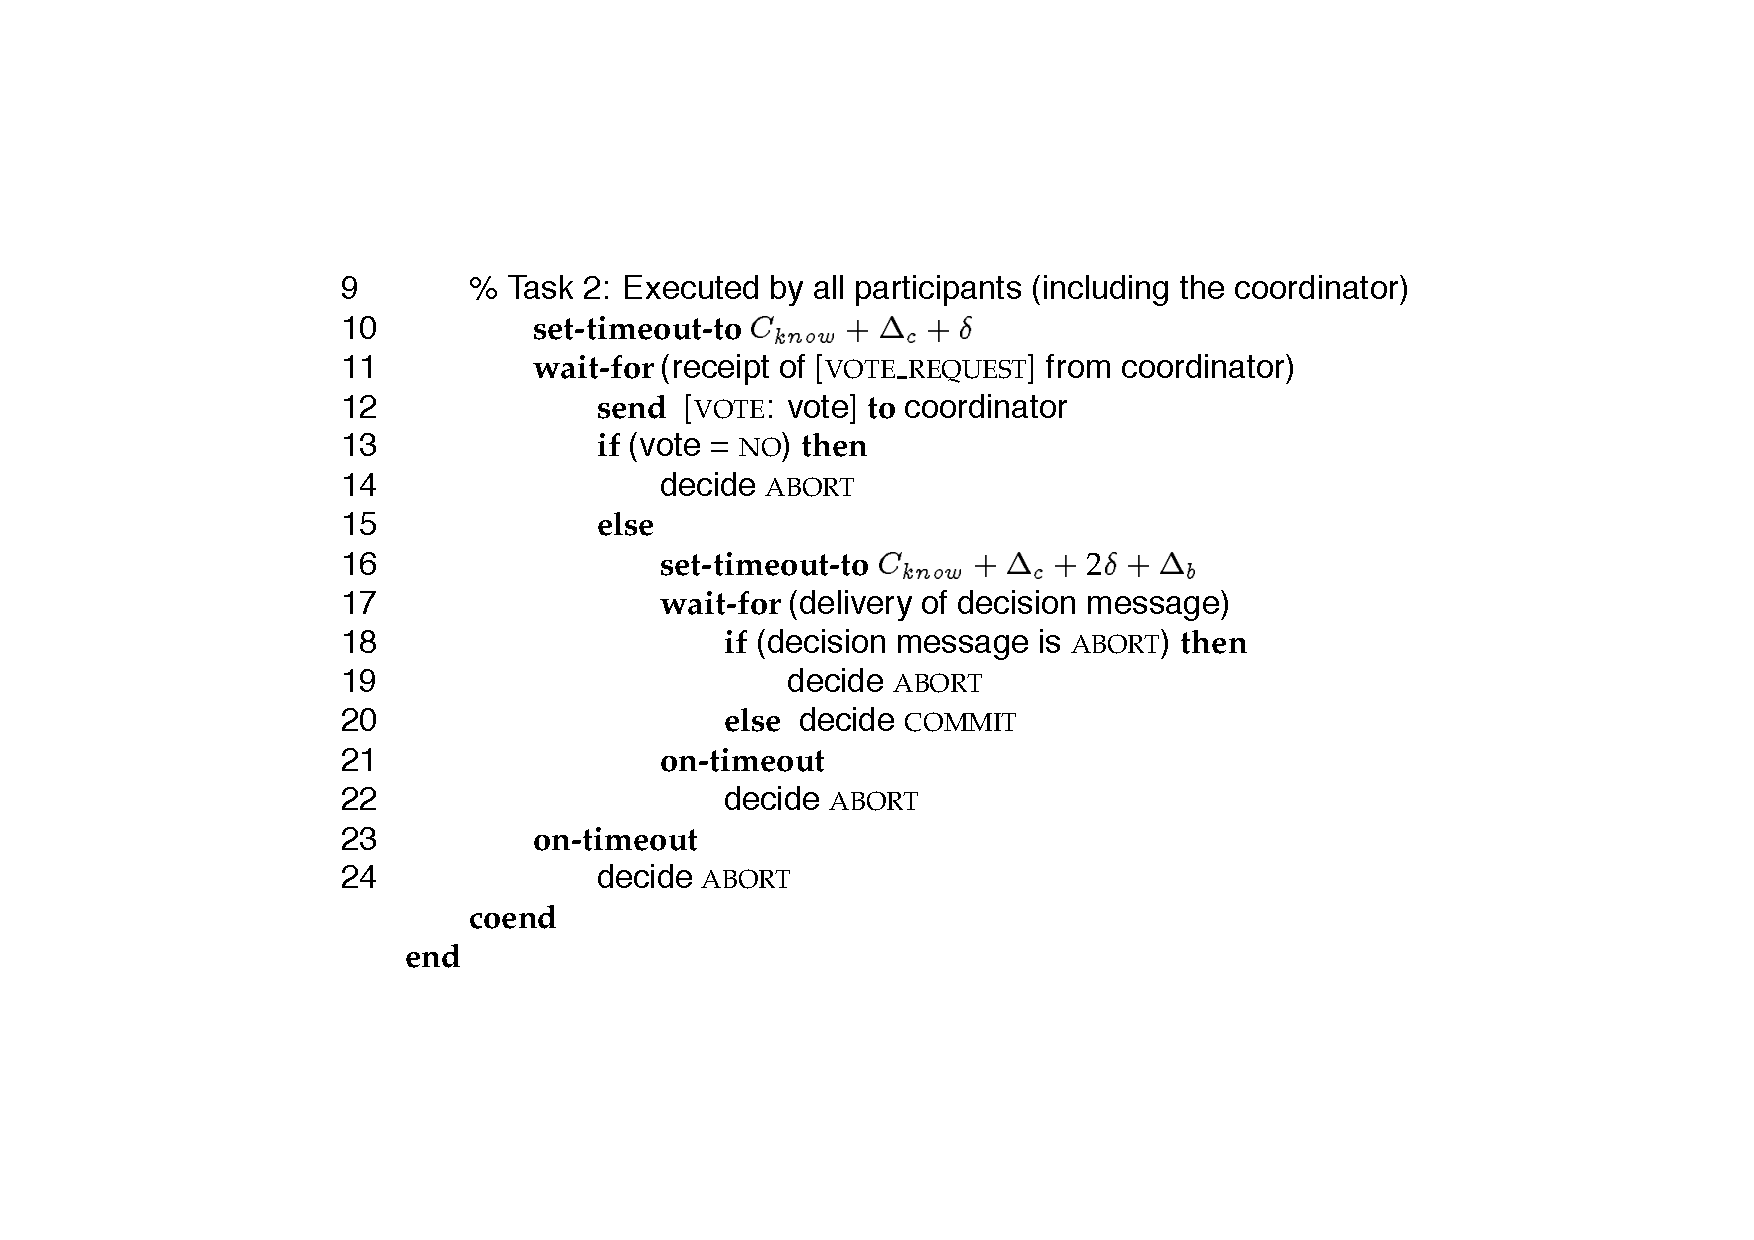
\includegraphics[width=\textwidth]{alg3.pdf}

\end{frame}

%-------------------------------------------------------------------------
\begin{frame}{ACP - UTRB}

\begin{block}{ACP - UTRB}	
If we use UTRB instead of TBEB, we obtain ACP-UTRB, which is equivalent to 3PC.
\end{block}

\bigskip

\bigskip
\begin{block}{Correctness}
The termination protocol is not needed any more.

\smallskip
Proof:
\BI
\item AC1-AC4: only AC1 is changed from before, we need to prove that $q$ cannot decide \ABORT\ in line 22
\item AC5: By the structure of the protocol, each line we have a decide
\EI
\end{block}
 
\end{frame}
 
  

%-------------------------------------------------------------------------
\begin{frame}{ACP - UTRB – Performance}
	
\BI	
\item ACP- BEB
	\BI
	\item  $4n$ total messages
	\item   $n$ invoker-to-all
	\item   $n$ coordinator-to-all
	\item   $n$ all-to-coordinator
	\item   $n$ coordinator-to-all
	\EI
\smallskip
\item ACP-UTRB
	\BI
	\item   $3n + n^2$ total messages
	\item   $n$ invoker-to-all
	\item   $n$ coordinator-to-all
	\item   $n$ all-to-coordinator
	\item   $n^2$ all-to-all
	\EI
\EI
\end{frame}

%-------------------------------------------------------------------------
\begin{frame}{Recovery}

\BI
\item To conclude, we need to consider the possibility of a participant that was down becoming operational after being repaired
\EI

\begin{block}{Recovery protocol}
  \BI
  \item During normal execution, log all “transactional events” in a \alert{distributed transaction log} (dt-log)
  	\BI
  	\item \textsc{t-start}, \textsc{vote yes}, \textsc{vote no}, \COMMIT, \ABORT
  	\EI
  \item At recovery, try to conclude all transactions that were in progress at the participant at the time of crash
  \item If recovery is not possible by simply looking at the log, try to get help from other participants
  \EI
\end{block}
  

\end{frame}

%-------------------------------------------------------------------------
\begin{frame}{Recovery protocol}

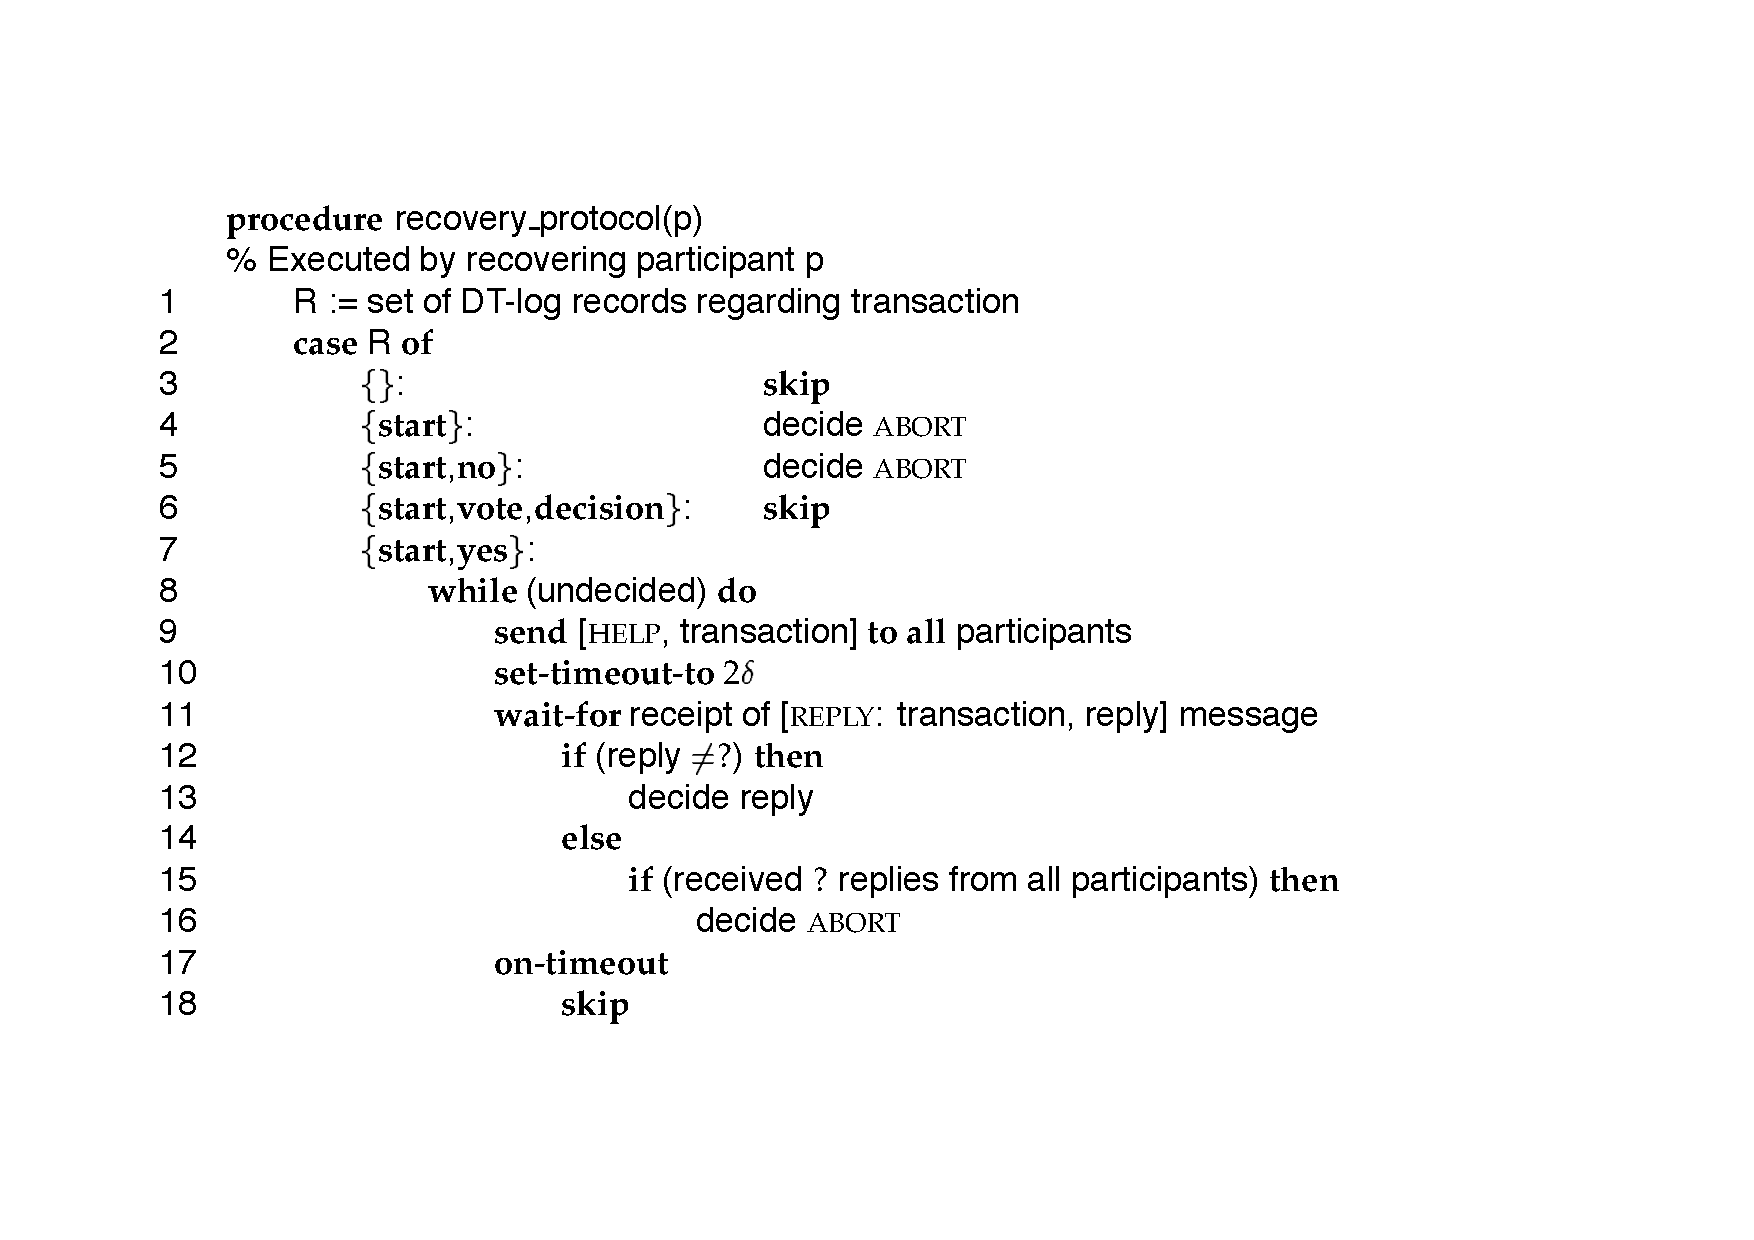
\includegraphics[width=0.90\textwidth]{alg4.pdf}

\end{frame}

%-------------------------------------------------------------------------
\begin{frame}{Recovery protocol}
	
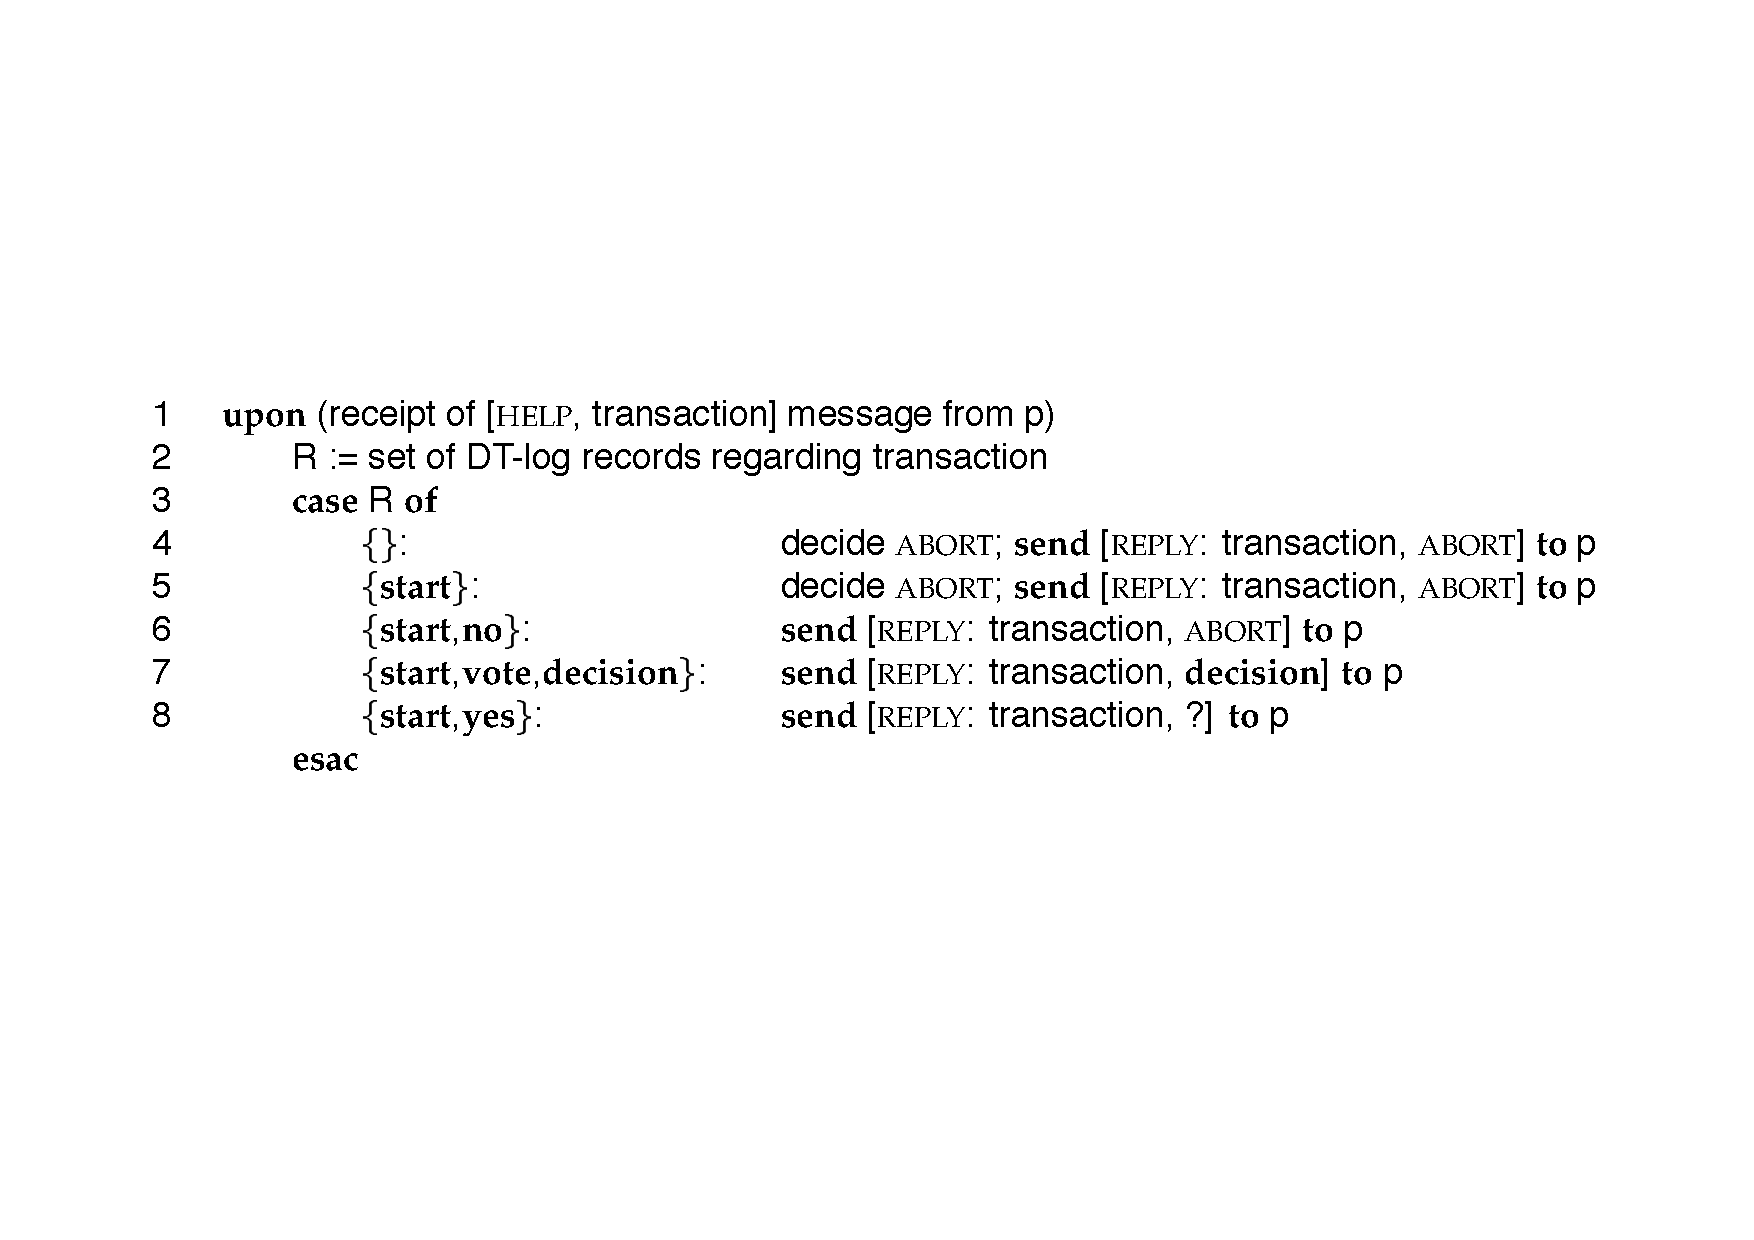
\includegraphics[width=\textwidth]{alg5.pdf}
	
\end{frame}

%%%%%%%%%%%%%%%%%%%%%%%%%%%%%%%%%%%%%%%%%%%%%%%%%%%%%%%%%%%%%%%%%%%%%%%%%%

%-------------------------------------------------------------------------
\begin{RMFrame}

\BI
\item \bibentry{babaoglu93understanding}
\EI

\end{RMFrame}


\end{document}